
\section{Methodology}

\subsection{Tasks}
\label{sec:tasks}

We evaluate on a diverse set of classification tasks representative of different modalities.
In particular, we are interested in if language models are inherently capable of \emph{universal computation}, by which we mean the ability to learn representations for predictive learning across diverse modalities.

\textbf{Bit memory.}
Similar to the task proposed by \cite{miconi2018hebbian}, we consider a bit memory task where the model is shown 5 bitstrings each of length 1000.
Afterwards, the model is shown a masked version of one of the bitstrings, where each bit is masked with probability $0.5$, and the model is tasked with producing the original bitstring.
The bitstrings are broken up into sequences of length 50, so that the models are fed 120 tokens of dimension 50.

\textbf{Bit XOR.}
Similar to the bit memory task, the model is shown 2 bitstrings of length 5, where the model must predict the element-wise XOR of the two bitstrings.
The bitstrings are shown 1 bit at a time, so the models are fed 10 tokens of dimension 1.

\textbf{ListOps.}
Taken from \cite{tay2020lra}, the model is shown a sequence of list operations (ex. \texttt{[ MAX 4 3 [ MIN 2 3 ] 1 0 ]}) and tasked with predicting the resulting output digit (ex. \texttt{4}).
This task evaluates the ability of a model to parse mathematical expressions and evaluate over a long context.
The model is shown 1 token at a time, so the models are fed 512 tokens of dimension 15.

\textbf{MNIST.}
We use the standard MNIST benchmark, where the model must classify a handwritten digit from a $32 \times 32$ black-and-white image.
The tokens given to the model are $4 \times 4$ image patches, so the models are fed 64 tokens of dimension 16.

\textbf{CIFAR-10.}
We use the standard CIFAR-10 benchmark \citep{krizhevsky2009cifar}, where the tokens given to the model are $4 \times 4$ image patches, so the models are fed 64 tokens of dimension 16.

\textbf{CIFAR-10 LRA.}
This is a modified version of the above task taken from the Long Range Arena benchmark where the images are converted to grayscale and flattened with a token length of 1 \citep{tay2020lra}.
As a result, the input sequence consists of 1024 tokens of dimension 1.
This task is much more challenging than vanilla CIFAR-10 classification above as the models must learn patterns over a significantly longer sequence length and have minimal spatial inductive bias.

\textbf{Remote homology detection.}
In this task, we are interested in predicting the fold for a protein, represented as an amino acid sequence.
We use the datasets provided by TAPE \citep{rap2019tape, fox2013scop, hou2018deepsf}, where the train/test split is generated by holding out certain evolutionary groups.
Note that we do not pretrain on Pfam \citep{elgebali2019pfam}, which is common in other works.
There are 20 common and 5 uncommon amino acids (25 different types of inputs), and there are 1195 possible labels to predict.
We only consider sequences of length less than 1024 for simplicity.
The models are thus fed up to 1024 tokens of dimension 25.

\subsection{Architecture}
\label{sec:architecture}

\begin{figure}
    \centering
    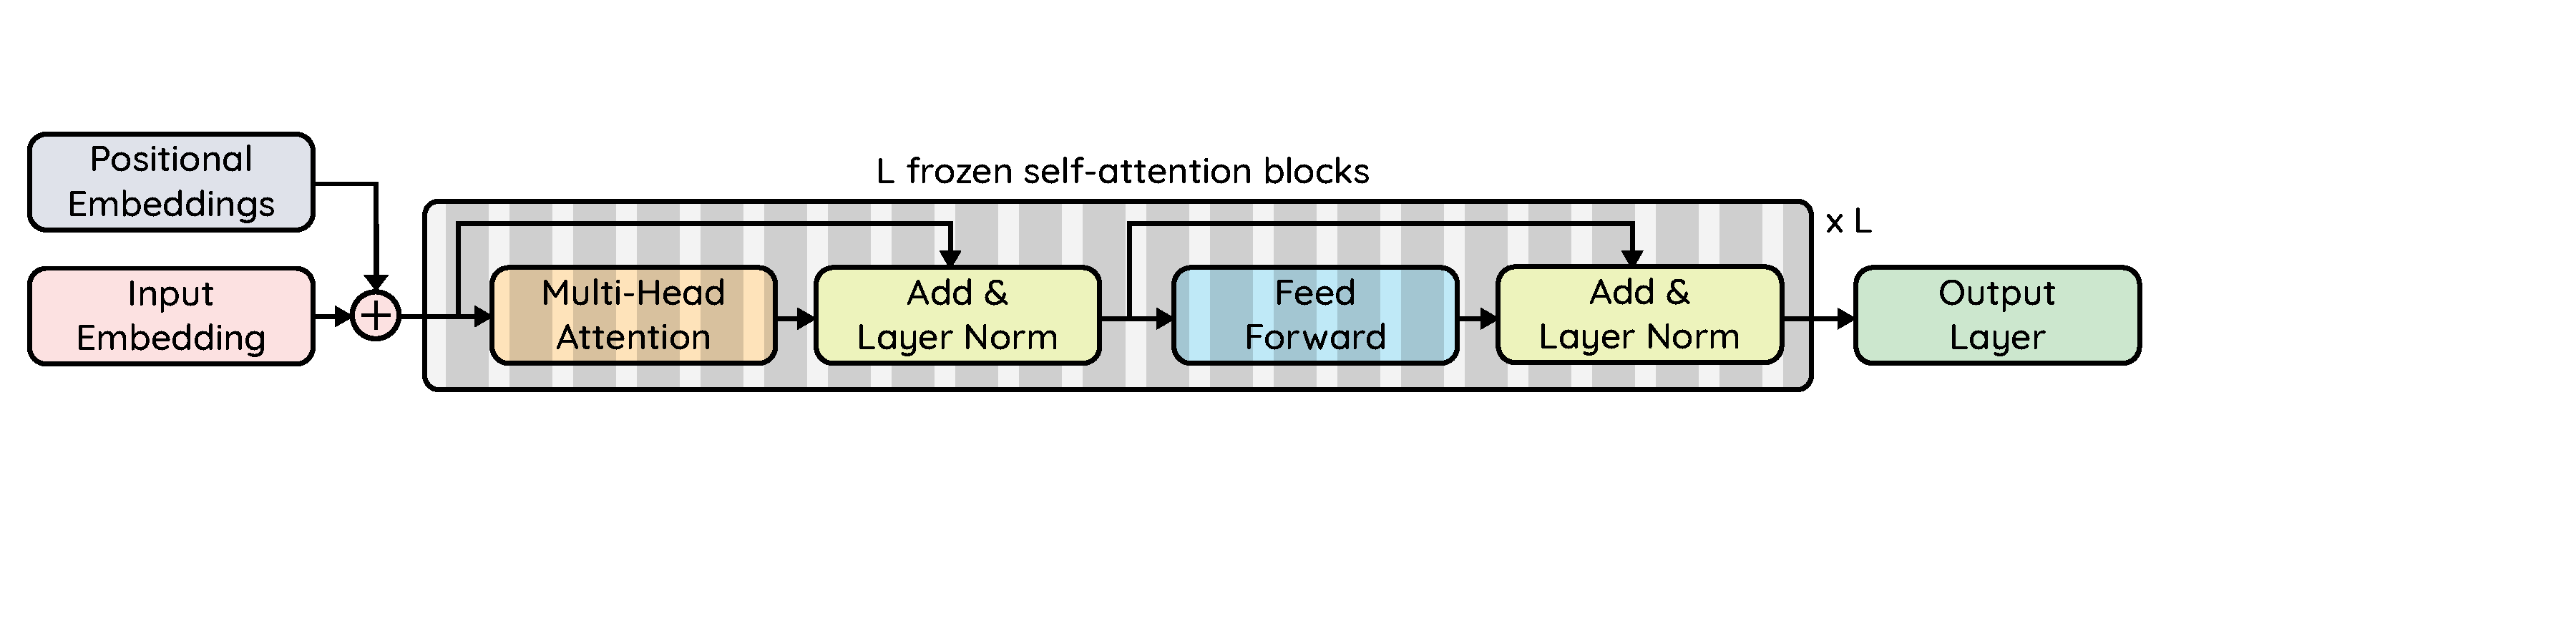
\includegraphics[width=1\linewidth]{figures/architecture/architecture.pdf}
    
    \caption{
        Frozen Pretrained Transformer (FPT).
        The self-attention \& feedforward layers are frozen.
    }
    \label{fig:architecture}
\end{figure}

The architecture we use is summarized in Figure \ref{fig:architecture}.
Denote the embedding size/hidden dimension of the transformer as $n_{dim}$, the number of layers as $n_{layers}$, (note $n_{dim} = 768$ and $n_{layers} = 12$ for the base size models), the input dimension as $d_{in}$, the output dimension (number of classes) as $d_{out}$, and the maximum length of the sequence as $l$.
We consider finetuning the following parameters of a pretrained GPT-2 model \citep{radford2019gpt2}:

\begin{itemize}[leftmargin=*]
    \item \textbf{Output layer:} it is crucial to finetune the output layer since we are transferring to a completely new task -- we use the simplest possible instantiation of an output network, being a single linear layer applied to the last output token output by the transformer, in order to highlight that almost all the computation is being performed by the frozen transformer.
    The output layer has $n_{dim} \times d_{out}$ parameters for the weight matrix.
    For example, for the base models on CIFAR-10, this comes out to $768 \cdot 10 = 7680$ parameters.

    \item \textbf{Input layer:} it is important to reinitialize a new input layer since we are reading in a new modality; in essence, we are learning how to query the transformer.
    This contrasts with prior unsupervised embedding evaluation techniques, such as linear probing -- due to the change in modality, we instead should train the input layer as well, and evaluate if the frozen intermediate transformer model performs effective computation.
    Again, we use a linear layer to minimize the amount of computation outside the transformer.
    The input layer has $d_{in} \times n_{dim}$ parameters for the weight matrix/embeddings, and an additional $n_{dim}$ parameters if there is a bias term.
    For the base models on CIFAR-10, this comes out to $16 \cdot 768 = 13056$ parameters.
    
    \item \textbf{Layer norm parameters:} as is standard practice in other finetuning works \citep{rebuffi2017adapter, houlsby2019adapter}, we also finetune the affine layer norm parameters (scale and bias), which adapt to the statistics of the downstream task in a new domain.
    % , allowing normalization on the new domain.
    In GPT-2, layer norm is applied twice per block, so these are a total of $4 \times n_{dim} \times n_{layers}$ parameters.
    For the base models on CIFAR-10, these come out to $4 \cdot 768 \cdot 12 = 36684$ parameters.
    
    \item \textbf{Positional embeddings:} While we observe that positional embeddings can be surprisingly universal between modalities (see Section \ref{sec:params}), we generally see a small benefit to finetuning the positional embeddings which have a cheap parameter cost of $l \times n_{dim}$.
    For the base models on CIFAR-10, these come out to $64 \cdot 768 = 49512$ parameters.
\end{itemize}
\vspace{2em}

Given the cheap linear scaling of these parameters, the parameter counts of large transformer models are dominated by the quadratic (in $n_{dim}$ and $l$) self-attention and feedforward layers.
For the base CIFAR-10 model with 124M parameters, these come out to approximately $0.086\%$ of the network.
Due to this scaling, this number decreases with larger model sizes, down to $0.029\%$ of the GPT-2 XL model.
We further ablate the importance of each parameter in Section \ref{sec:params}.
For more details and a description of the architecture, see Appendix \ref{app:architecture}.

Note that, crucially, all communication between tokens in the model are frozen.
The data in each datapoint is chunked into discrete tokens (bits, image patches, amino acids, etc.), and can only reference each other via the frozen attention connections, which are not trained; additionally, neither the output nor the input layers are connected to multiple tokens.
Our key investigation is to analyze the computation that is already inherent in the language model, and hence we do a minimal amount of computation that is learned on the downstream modality.
